\documentclass{standalone}
\usepackage{tikz}
\usetikzlibrary{patterns, positioning}


\begin{document}
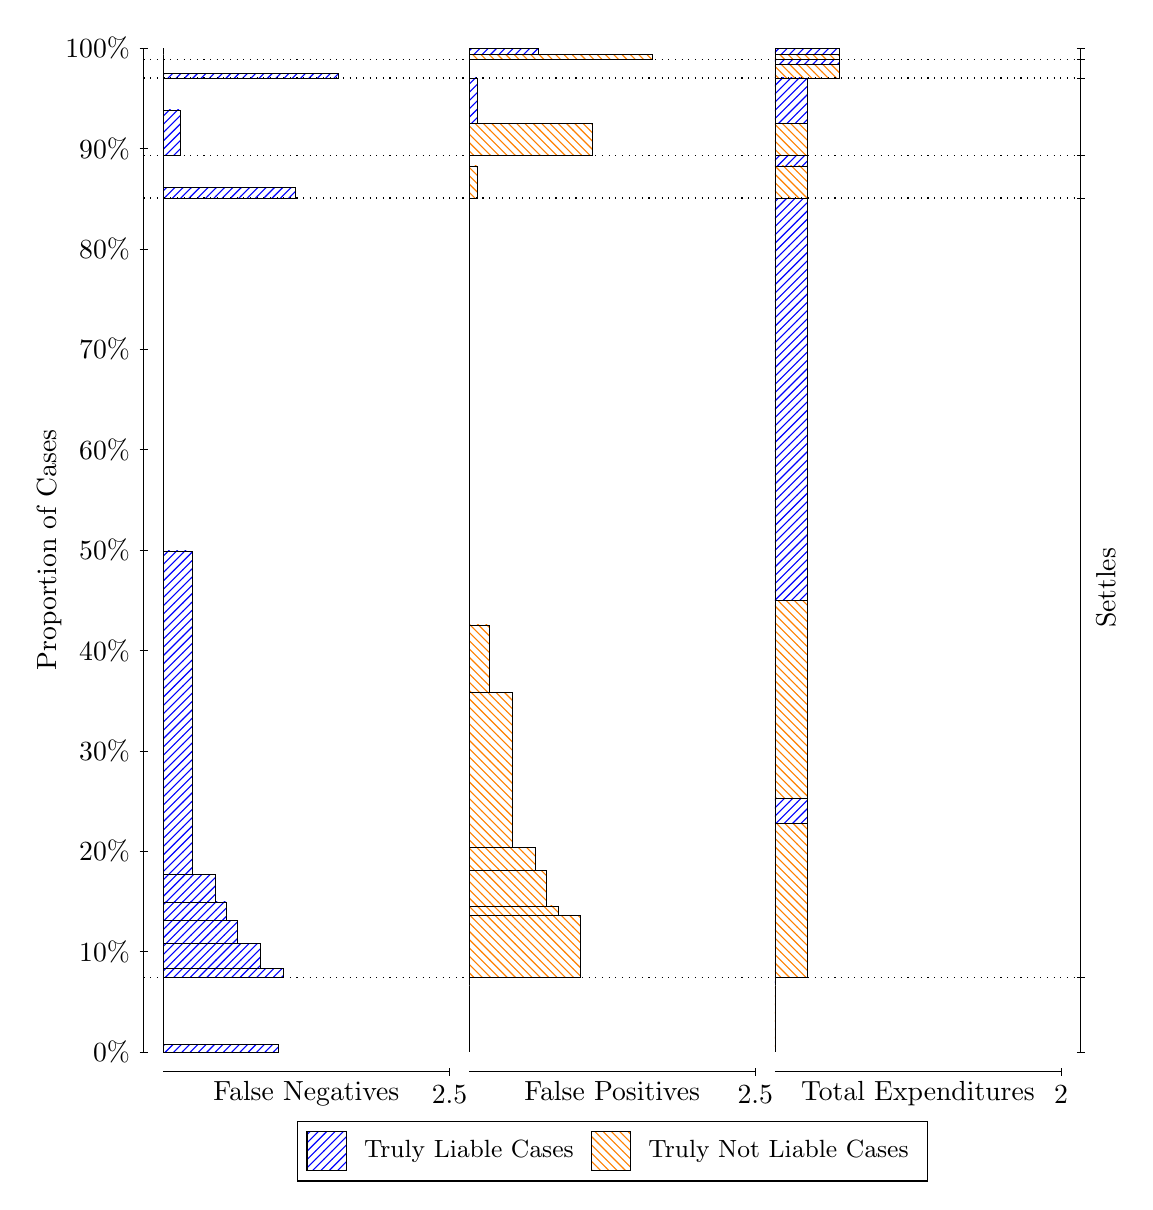
\begin{tikzpicture}
\draw[black, very thin] (1.5,1.75) -- (1.5,14.5);
\node[rotate=90, text=black, anchor=center] at (0.3, 8.125) {Proportion of Cases};
\draw[black, very thin] (1.45,1.75) -- (1.55,1.75);
\node[text=black, anchor=east] at (1.45, 1.75) {0\%};
\draw[black, very thin] (1.45,3.025) -- (1.55,3.025);
\node[text=black, anchor=east] at (1.45, 3.025) {10\%};
\draw[black, very thin] (1.45,4.3) -- (1.55,4.3);
\node[text=black, anchor=east] at (1.45, 4.3) {20\%};
\draw[black, very thin] (1.45,5.575) -- (1.55,5.575);
\node[text=black, anchor=east] at (1.45, 5.575) {30\%};
\draw[black, very thin] (1.45,6.85) -- (1.55,6.85);
\node[text=black, anchor=east] at (1.45, 6.85) {40\%};
\draw[black, very thin] (1.45,8.125) -- (1.55,8.125);
\node[text=black, anchor=east] at (1.45, 8.125) {50\%};
\draw[black, very thin] (1.45,9.4) -- (1.55,9.4);
\node[text=black, anchor=east] at (1.45, 9.4) {60\%};
\draw[black, very thin] (1.45,10.675) -- (1.55,10.675);
\node[text=black, anchor=east] at (1.45, 10.675) {70\%};
\draw[black, very thin] (1.45,11.95) -- (1.55,11.95);
\node[text=black, anchor=east] at (1.45, 11.95) {80\%};
\draw[black, very thin] (1.45,13.225) -- (1.55,13.225);
\node[text=black, anchor=east] at (1.45, 13.225) {90\%};
\draw[black, very thin] (1.45,14.5) -- (1.55,14.5);
\node[text=black, anchor=east] at (1.45, 14.5) {100\%};

\draw[black, very thin] (13.4,1.75) -- (13.4,14.5);
\draw[black, very thin] (13.35,1.75) -- (13.45,1.75);
\node[anchor=west] at (13.35, 1.75) {};
\draw[black, very thin] (13.35,2.6924) -- (13.45,2.6924);
\node[anchor=west] at (13.35, 2.6924) {};
\draw[black, very thin] (13.35,12.595) -- (13.45,12.595);
\node[anchor=west] at (13.35, 12.595) {};
\draw[black, very thin] (13.35,13.139) -- (13.45,13.139);
\node[anchor=west] at (13.35, 13.139) {};
\draw[black, very thin] (13.35,14.12) -- (13.45,14.12);
\node[anchor=west] at (13.35, 14.12) {};
\draw[black, very thin] (13.35,14.359) -- (13.45,14.359);
\node[anchor=west] at (13.35, 14.359) {};
\draw[black, very thin] (13.35,14.5) -- (13.45,14.5);
\node[anchor=west] at (13.35, 14.5) {};

\draw[black, very thin, pattern color=blue, pattern=north east lines] (1.75,1.75) rectangle (3.2033,1.8491);
\draw[black, very thin, pattern color=orange, pattern=north west lines] (1.75,1.8491) rectangle (1.75,2.6924);
\draw[black, very thin, pattern color=blue, pattern=north east lines] (1.75,2.6924) rectangle (3.276,2.8127);
\draw[black, very thin, pattern color=blue, pattern=north east lines] (1.75,2.8127) rectangle (2.9853,3.128);
\draw[black, very thin, pattern color=blue, pattern=north east lines] (1.75,3.128) rectangle (2.6947,3.4208);
\draw[black, very thin, pattern color=blue, pattern=north east lines] (1.75,3.4208) rectangle (2.5493,3.6559);
\draw[black, very thin, pattern color=blue, pattern=north east lines] (1.75,3.6559) rectangle (2.404,4.0073);
\draw[black, very thin, pattern color=blue, pattern=north east lines] (1.75,4.0073) rectangle (2.1133,8.1133);
\draw[black, very thin, pattern color=orange, pattern=north west lines] (1.75,8.1133) rectangle (1.75,12.595);
\draw[black, very thin, pattern color=blue, pattern=north east lines] (1.75,12.595) rectangle (3.4213,12.732);
\draw[black, very thin, pattern color=orange, pattern=north west lines] (1.75,12.732) rectangle (1.75,13.139);
\draw[black, very thin, pattern color=blue, pattern=north east lines] (1.75,13.139) rectangle (1.968,13.715);
\draw[black, very thin, pattern color=orange, pattern=north west lines] (1.75,13.715) rectangle (1.75,14.12);
\draw[black, very thin, pattern color=blue, pattern=north east lines] (1.75,14.12) rectangle (3.9663,14.18);
\draw[black, very thin, pattern color=orange, pattern=north west lines] (1.75,14.18) rectangle (1.75,14.359);
\draw[black, very thin, pattern color=orange, pattern=north west lines] (1.75,14.359) rectangle (1.75,14.418);
\draw[black, very thin, pattern color=blue, pattern=north east lines] (1.75,14.418) rectangle (1.75,14.5);
\draw[black, very thin, pattern color=orange, pattern=north west lines] (5.6333,1.75) rectangle (5.6333,2.5932);
\draw[black, very thin, pattern color=blue, pattern=north east lines] (5.6333,2.5932) rectangle (5.6333,2.6924);
\draw[black, very thin, pattern color=orange, pattern=north west lines] (5.6333,2.6924) rectangle (7.0503,3.4816);
\draw[black, very thin, pattern color=orange, pattern=north west lines] (5.6333,3.4816) rectangle (6.7597,3.6048);
\draw[black, very thin, pattern color=orange, pattern=north west lines] (5.6333,3.6048) rectangle (6.6143,4.0536);
\draw[black, very thin, pattern color=orange, pattern=north west lines] (5.6333,4.0536) rectangle (6.469,4.3511);
\draw[black, very thin, pattern color=orange, pattern=north west lines] (5.6333,4.3511) rectangle (6.1783,6.3149);
\draw[black, very thin, pattern color=orange, pattern=north west lines] (5.6333,6.3149) rectangle (5.8877,7.1743);
\draw[black, very thin, pattern color=blue, pattern=north east lines] (5.6333,7.1743) rectangle (5.6333,12.595);
\draw[black, very thin, pattern color=orange, pattern=north west lines] (5.6333,12.595) rectangle (5.7423,13.002);
\draw[black, very thin, pattern color=blue, pattern=north east lines] (5.6333,13.002) rectangle (5.6333,13.139);
\draw[black, very thin, pattern color=orange, pattern=north west lines] (5.6333,13.139) rectangle (7.1957,13.544);
\draw[black, very thin, pattern color=blue, pattern=north east lines] (5.6333,13.544) rectangle (5.7423,14.12);
\draw[black, very thin, pattern color=orange, pattern=north west lines] (5.6333,14.12) rectangle (5.6333,14.299);
\draw[black, very thin, pattern color=blue, pattern=north east lines] (5.6333,14.299) rectangle (5.6333,14.359);
\draw[black, very thin, pattern color=orange, pattern=north west lines] (5.6333,14.359) rectangle (7.9587,14.418);
\draw[black, very thin, pattern color=blue, pattern=north east lines] (5.6333,14.418) rectangle (6.5053,14.5);
\draw[black, very thin, pattern color=orange, pattern=north west lines] (9.5167,1.75) rectangle (9.5167,2.5932);
\draw[black, very thin, pattern color=blue, pattern=north east lines] (9.5167,2.5932) rectangle (9.5167,2.6924);
\draw[black, very thin, pattern color=orange, pattern=north west lines] (9.5167,2.6924) rectangle (9.9254,4.6562);
\draw[black, very thin, pattern color=blue, pattern=north east lines] (9.5167,4.6562) rectangle (9.9254,4.9715);
\draw[black, very thin, pattern color=orange, pattern=north west lines] (9.5167,4.9715) rectangle (9.9254,7.4896);
\draw[black, very thin, pattern color=blue, pattern=north east lines] (9.5167,7.4896) rectangle (9.9254,12.595);
\draw[black, very thin, pattern color=orange, pattern=north west lines] (9.5167,12.595) rectangle (9.9254,13.002);
\draw[black, very thin, pattern color=blue, pattern=north east lines] (9.5167,13.002) rectangle (9.9254,13.139);
\draw[black, very thin, pattern color=orange, pattern=north west lines] (9.5167,13.139) rectangle (9.9254,13.544);
\draw[black, very thin, pattern color=blue, pattern=north east lines] (9.5167,13.544) rectangle (9.9254,14.12);
\draw[black, very thin, pattern color=orange, pattern=north west lines] (9.5167,14.12) rectangle (10.334,14.299);
\draw[black, very thin, pattern color=blue, pattern=north east lines] (9.5167,14.299) rectangle (10.334,14.359);
\draw[black, very thin, pattern color=orange, pattern=north west lines] (9.5167,14.359) rectangle (10.334,14.418);
\draw[black, very thin, pattern color=blue, pattern=north east lines] (9.5167,14.418) rectangle (10.334,14.5);
\draw[black, dotted] (1.5,2.6924) -- (13.4,2.6924);
\draw[black, dotted] (1.5,12.595) -- (13.4,12.595);
\draw[black, dotted] (1.5,13.139) -- (13.4,13.139);
\draw[black, dotted] (1.5,14.12) -- (13.4,14.12);
\draw[black, dotted] (1.5,14.359) -- (13.4,14.359);
\draw[black, very thin] (1.75,1.5) -- (5.3833,1.5);
\node[text=black, anchor=north] at (3.5667, 1.5) {False Negatives};
\draw[black, very thin] (5.3833,1.45) -- (5.3833,1.55);
\node[text=black, anchor=north] at (5.3833, 1.45) {2.5};

\draw[black, very thin] (5.6333,1.5) -- (9.2667,1.5);
\node[text=black, anchor=north] at (7.45, 1.5) {False Positives};
\draw[black, very thin] (9.2667,1.45) -- (9.2667,1.55);
\node[text=black, anchor=north] at (9.2667, 1.45) {2.5};

\draw[black, very thin] (9.5167,1.5) -- (13.15,1.5);
\node[text=black, anchor=north] at (11.333, 1.5) {Total Expenditures};
\draw[black, very thin] (13.15,1.45) -- (13.15,1.55);
\node[text=black, anchor=north] at (13.15, 1.45) {2};


\node[text=black, centered, rotate=90] at (13.72, 7.6438) {Settles};





\draw (7.449999999999999,1.5) node[draw=none] (baseCoordinate) {};
\begin{scope}[align=center]
        \matrix[scale=0.5, draw=black, below=0.5cm of baseCoordinate, nodes={draw}, column sep=0.1cm]{
            \node[rectangle, draw, minimum width=0.5cm, minimum height=0.5cm, pattern color=blue, pattern=north east lines] {}; &
            \node[draw=none, font=\small, text=black] (B) {Truly Liable Cases}; &
            \node[rectangle, draw, minimum width=0.5cm, minimum height=0.5cm, pattern color=orange, pattern=north west lines] {}; &
            \node[draw=none, font=\small, text=black] (B) {Truly Not Liable Cases}; \\
            };
\end{scope}

\end{tikzpicture}
\end{document}